

\begin{figure}[h]
	\centering
	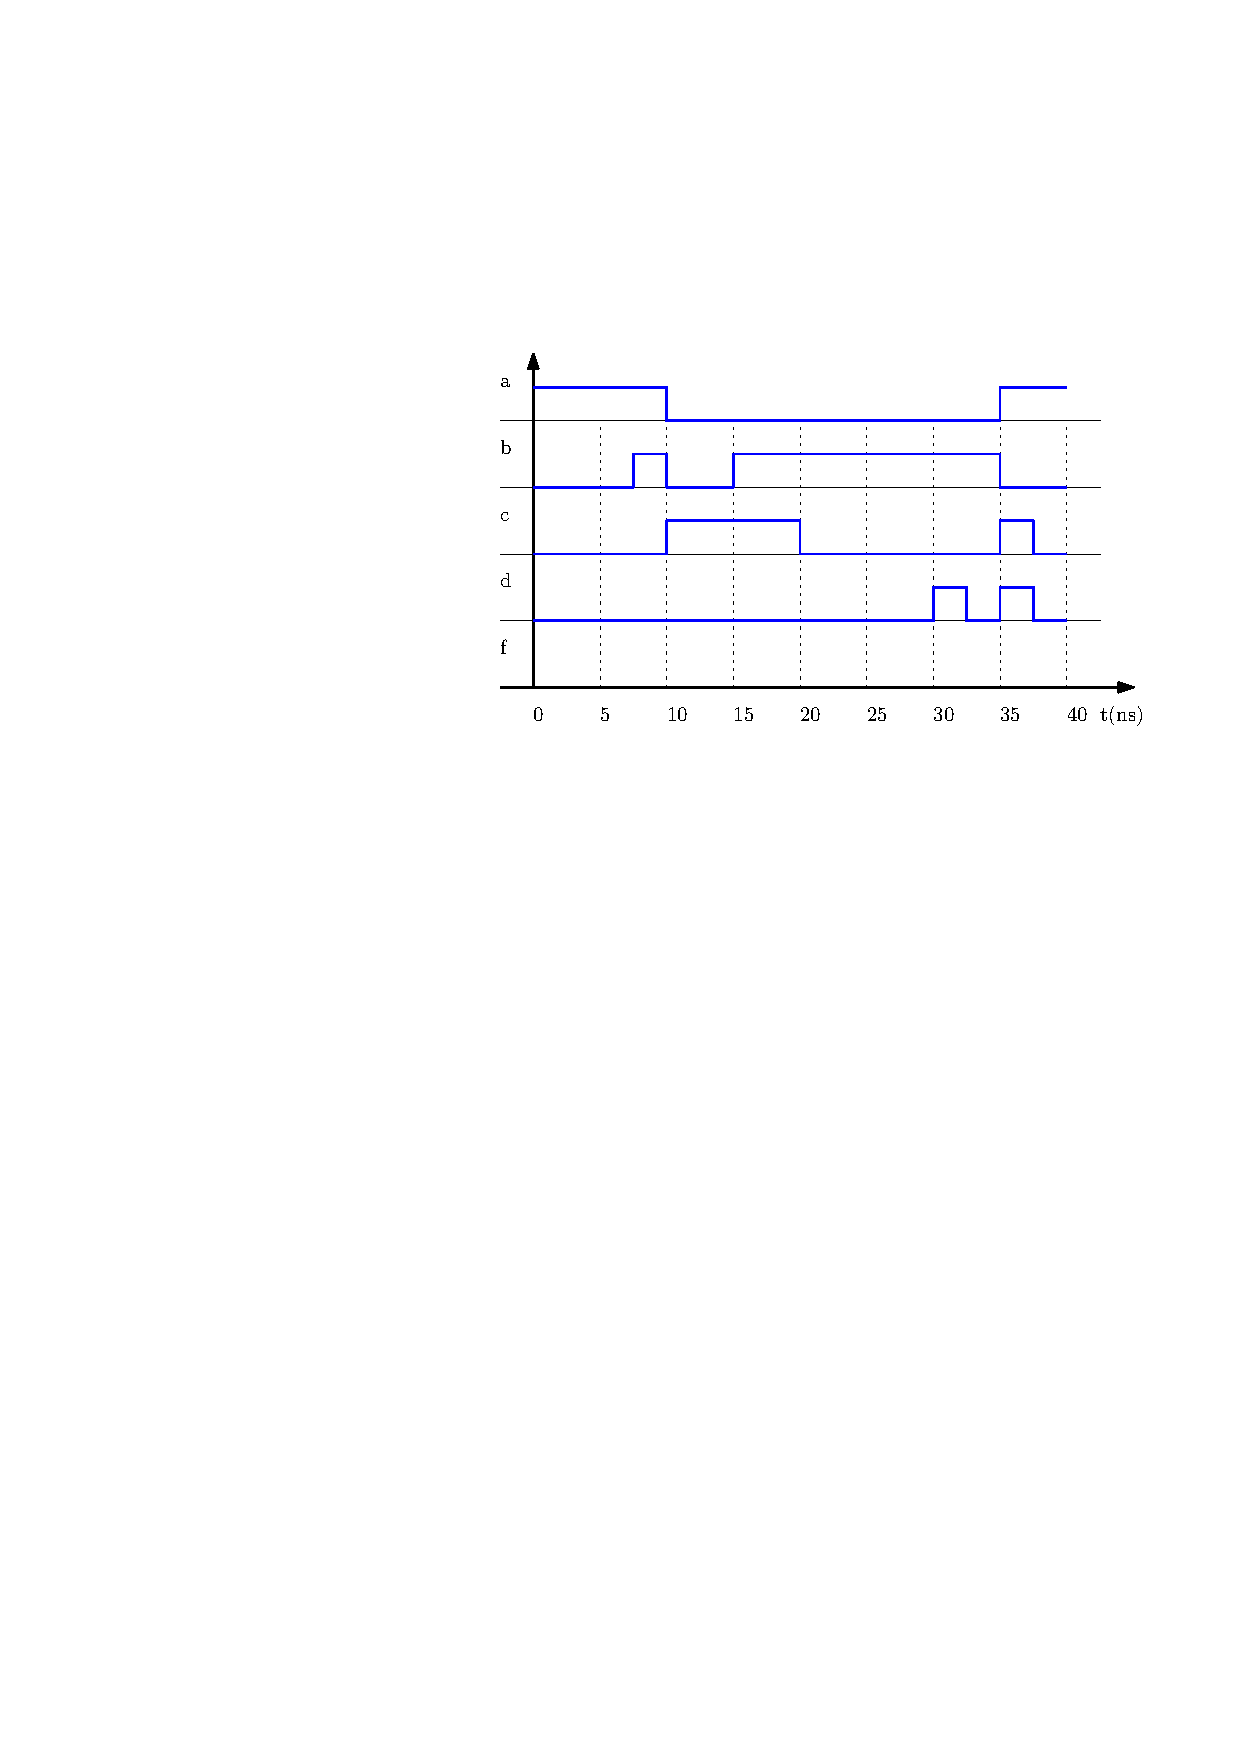
\includegraphics[width=0.5\textwidth]{fig/Q8.pdf}
	\caption{مدار طراحی شده سوال امتیازی ۱}
	\label{Qb1_Design}
\end{figure}

در شکل زیر نمودار خروجی را به‌ازای دو ورودی $A=00000000 $ و $B=11111111 $ تا $ A=00000001 $ و $B=11111111 $ را نشان می‌دهد.

\begin{figure}[h]
	\centering
	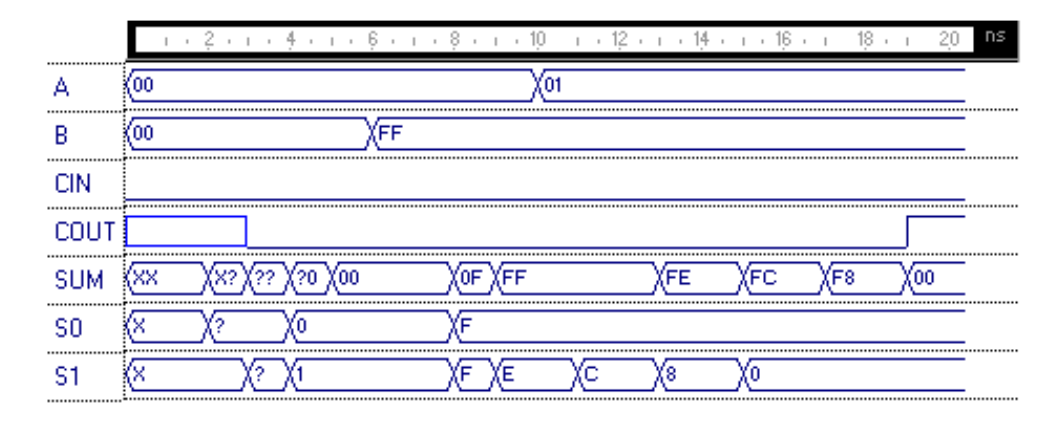
\includegraphics[width=0.9\textwidth]{fig/QB1_2.png}
	\caption{شکل موج خروجی مدار طراحی شده}
	\label{Qb1_2_Design}
\end{figure}